\documentclass[letterpaper, 12pt]{article}
\usepackage[margin=1in]{geometry}
\usepackage{graphicx}
\usepackage{listings}
\usepackage{circuitikz}
\graphicspath{{images/}{../Template/images/}}
\lstset{language=[Motorola68k]assembler,basicstyle=\ttfamily,frame=single}

\newcommand{\hwnumber}{Lab 2}
\newcommand{\duedate}{September 22nd, 2015}

\newcommand{\capper}{\begin{flushright}Aviles, Jean-Ralph \\ EEL3744 \\ Section 1539 \\ \duedate{} \\ \hwnumber{}\end{flushright}}

\begin{document}
\capper{}
\section*{Problems Encountered}
I messed up big time with my wire wrapping, broke a header and wire wrapped the switches and leds to the wrong ports. A lot of wasted time.
\section*{Future Work/Applications}
I can now wire-wrap and I have a better idea of how to design and code for additions to the uP board.
\section*{Appendix}
\subsection*{Part A}
\subsubsection*{Program to write to Port E simulated}
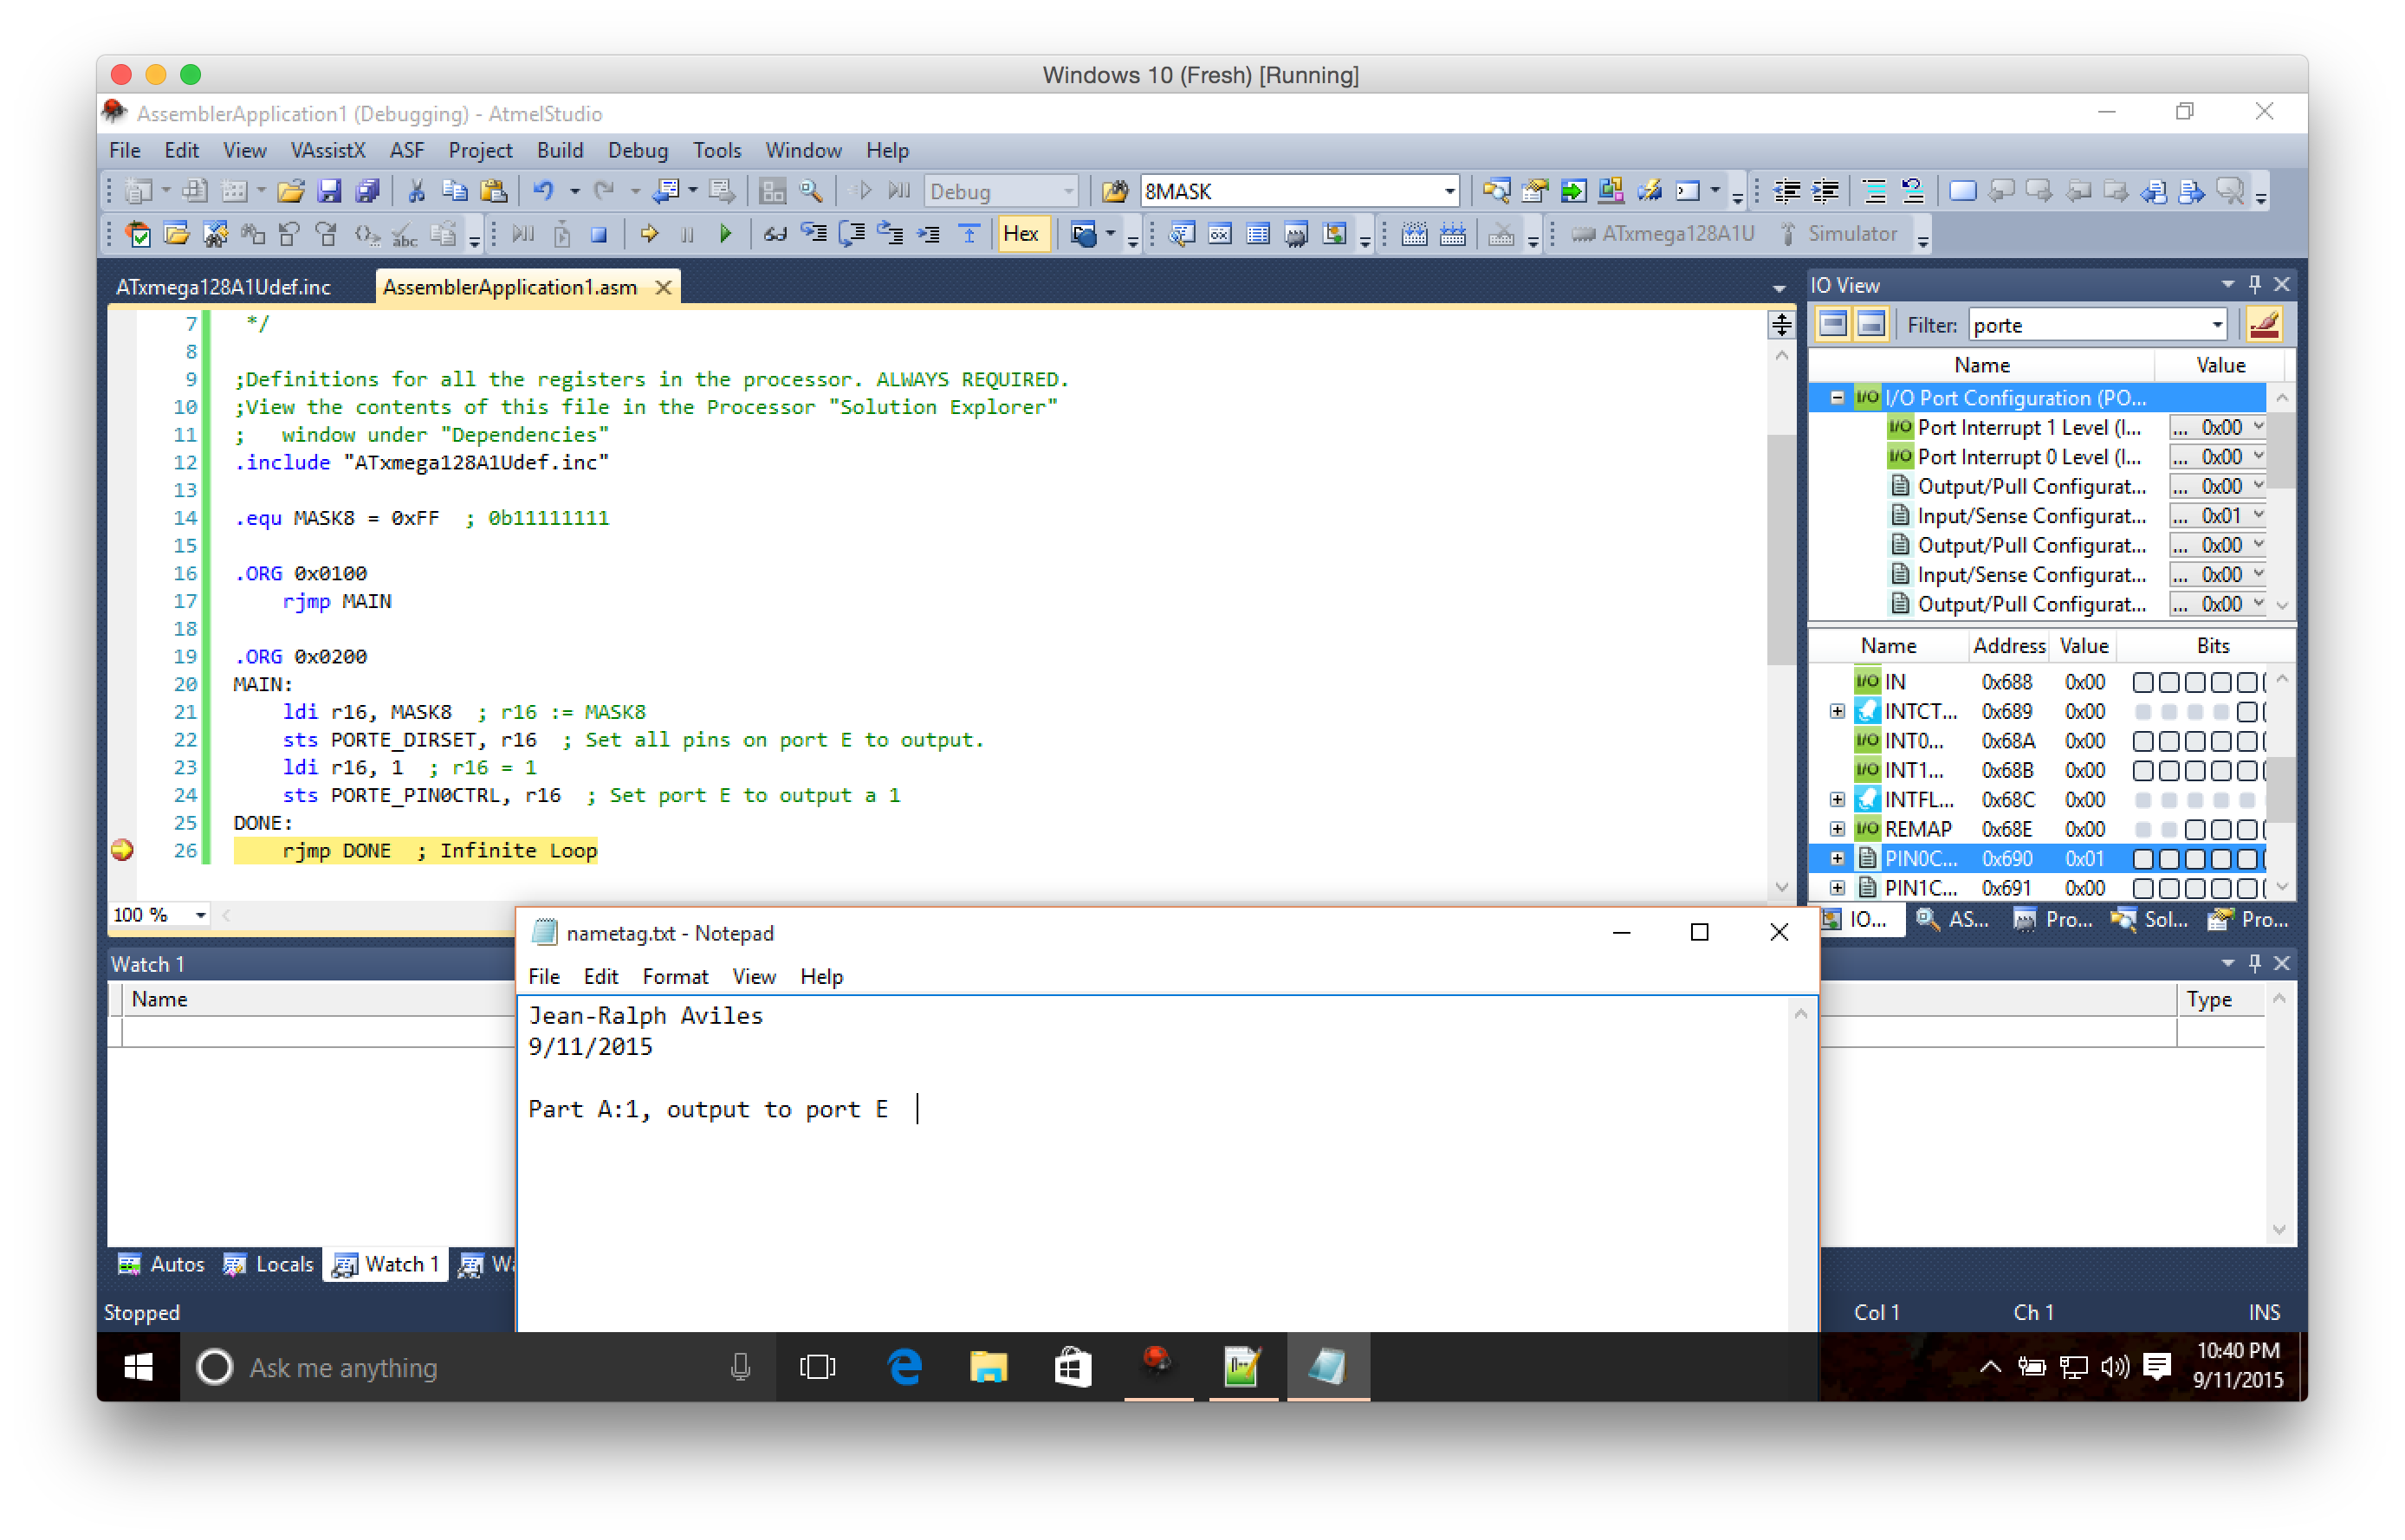
\includegraphics[width=\textwidth]{parta_1}
\subsubsection*{Program read from port F and write to Port E simulated}
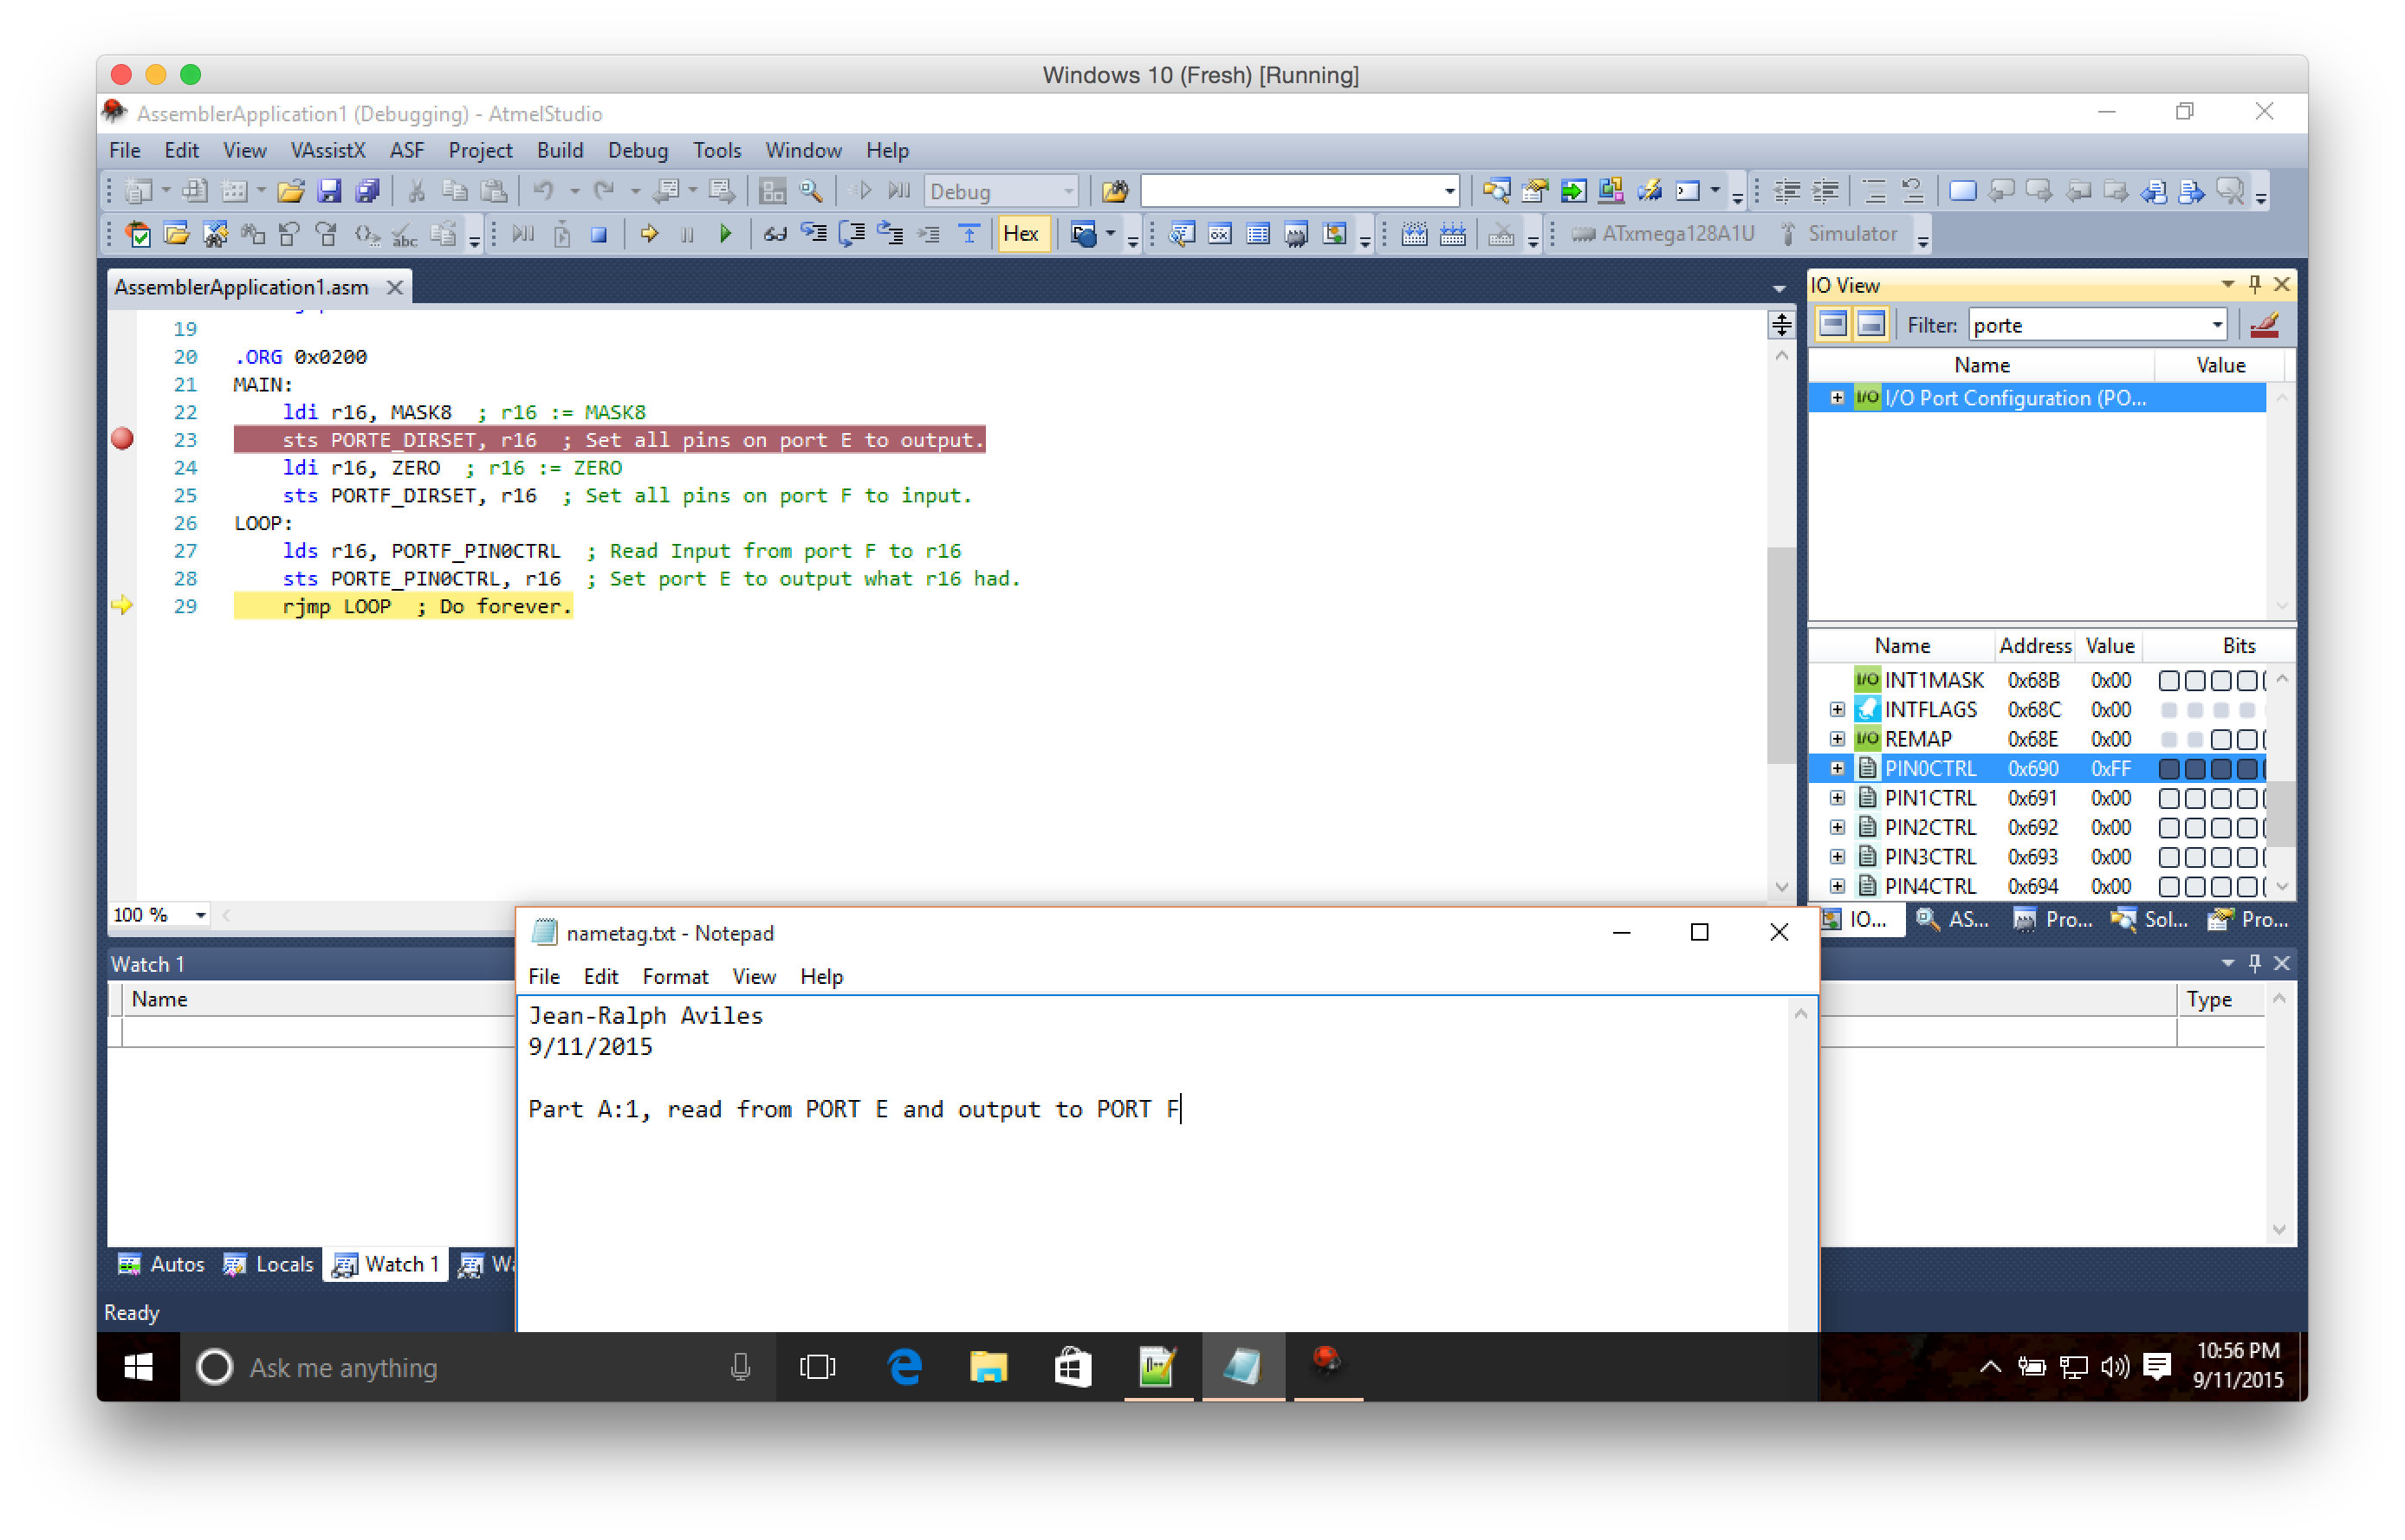
\includegraphics[width=\textwidth]{parta_2}
\subsection*{Part B}
\subsubsection*{Program to Blink LED at 2kHz}
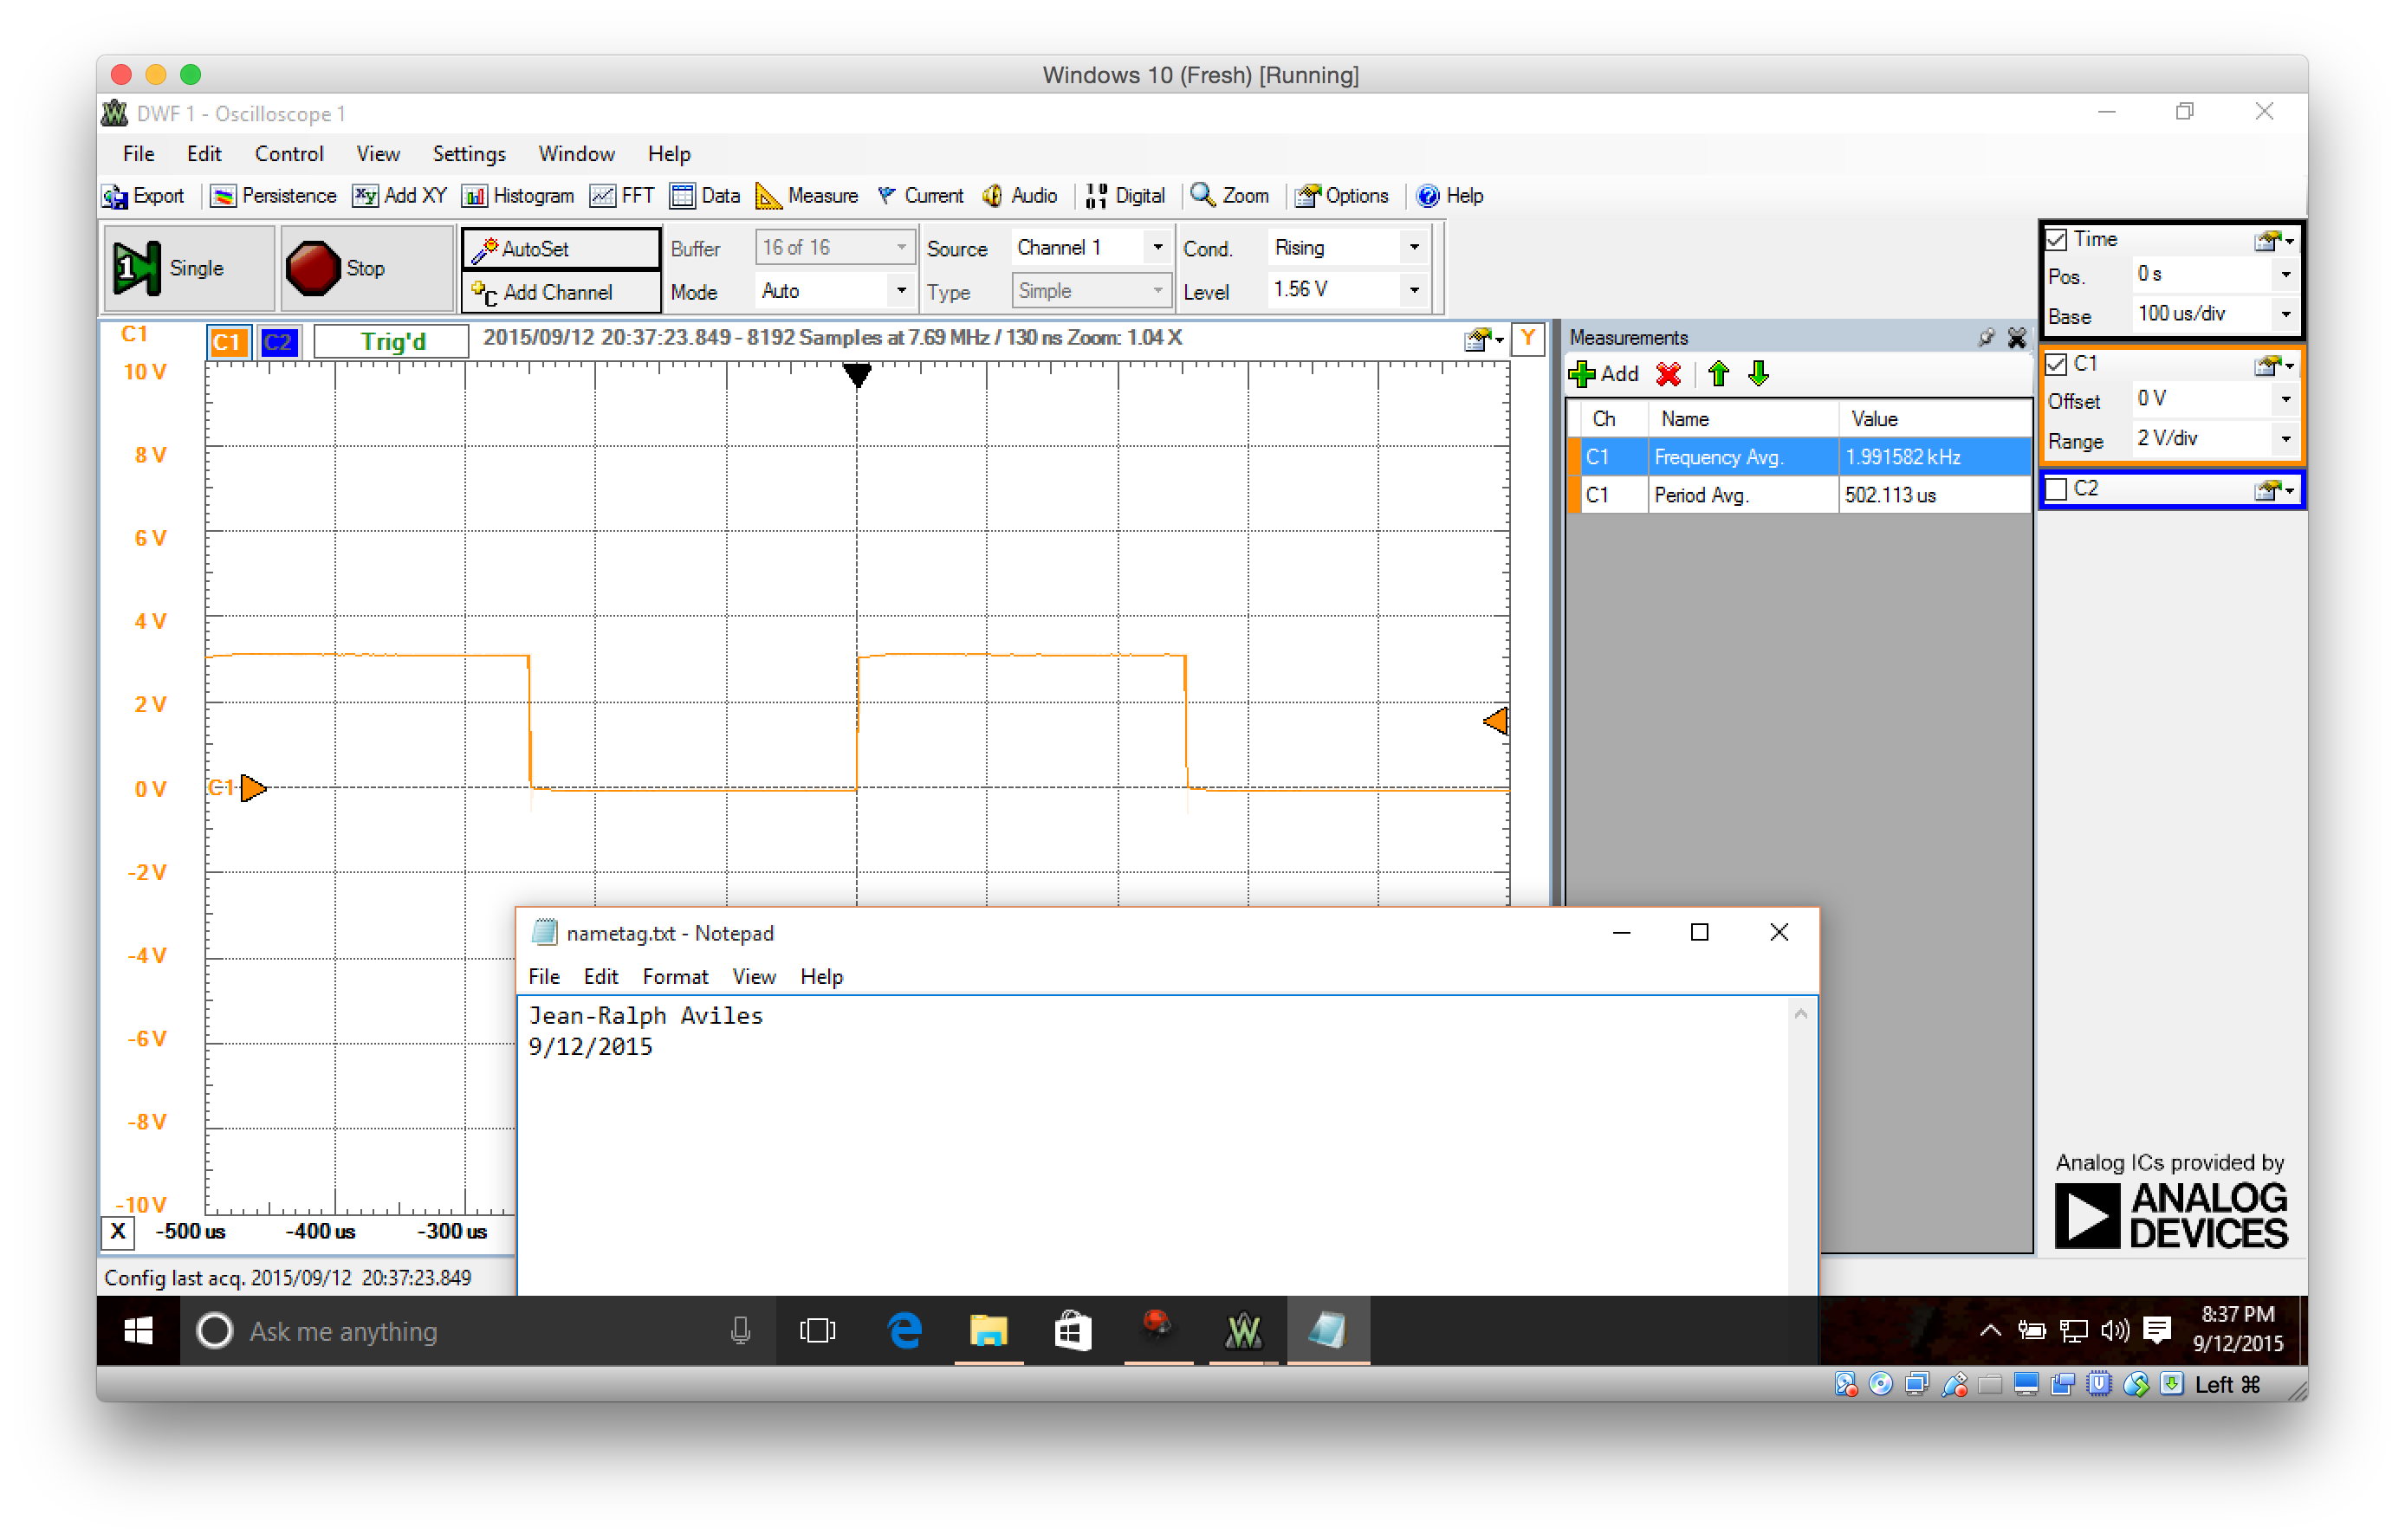
\includegraphics[width=\textwidth]{partb_1}
\section*{Pseudocode/Flowcharts}
\subsection*{Part A}
\subsubsection*{Program to write to Port E}
\lstinputlisting{code/parta_1.pc}
\subsubsection*{Program to read from Port F and read from Port E}
\lstinputlisting{code/parta_2.pc}
\subsubsection*{I/O Circuit Diagram}
\begin{center}
\begin{circuitikz}
\draw
(2, 0) to[generic, l=CPU] (2, -2) -- (0, -2)
       to[generic, l=PORT F] (0, -4)
       to[closing switch, l=IN(H)] (0, -5)
       to[R] (0, -6)
(0, -7) to[battery1, l=3.3V] (0, -6)
(2, -2) -- (4, -2)
       to[generic, l=PORT E] (4, -4)
       to[led, l=OUT(H)] (4, -5)
       to[R] (4, -6)
       node[ground]{} (4, -7);
\end{circuitikz}
\end{center}
\subsection*{Part B}
\subsubsection*{Program to Blink LED at 2kHz}
\lstinputlisting{code/partb_1.pc}
\subsection*{Part C}
\subsubsection*{Program for Part C}
\lstinputlisting{code/partc.pc}
\section*{Programs}
\subsection*{Part A}
\subsubsection*{Program to write to Port E}
\lstinputlisting{code/parta_1.asm}
\subsubsection*{Program to read from Port F and read from Port E}
\lstinputlisting{code/lab2a_JA.asm}
\subsection*{Part B}
\subsubsection*{Program to Blink LED at 2kHz}
\lstinputlisting{code/lab2b_JA.asm}
\subsection*{Part C}
\lstinputlisting{code/lab2c_JA.asm}
\end{document}
